% SOICT 2026 submission — Springer CCIS format (single-blind: keep author names).
% Requires the Springer LNCS/CCIS class `llncs.cls` + `splncs04.bst` from
% https://soict.org/wp-content/uploads/2025/09/Latex-Template-for-Springer.zip
% Max 12 pages excluding references. Figure: convert docs/paper/diagrams/soict_harlstmgat.svg -> PDF.
%
% VERSION 2026-09-04 (DRAFT). Primary quantitative results = VN30 + VN100 clean-data multi-horizon
% walk-forward (COMPLETE). The pooled/transfer VN30 ablation is now COMPLETE (all 4 horizons).
% HNX / HOSE / S&P 500 walk-forward and the estimator tables remain [provisional] / % TODO and must
% NOT be cited as final. All numbers are read from
% results/walkforward_volga/walkforward_volga_{vn30,vn100}_h{1,5,10,22}.json and
% results/pooled_transfer_vn30/pooled_vn30_h{1,5,10,22}.json (see soict_harlstmgat_2026-09-04_summary.md).
\documentclass[runningheads]{llncs}
\usepackage{graphicx}
\graphicspath{{diagrams/}}   % figure lives in docs/paper/diagrams/ (do NOT add ./ — collides with output pdf)
\usepackage{booktabs}
\usepackage{amsmath}
\usepackage{placeins}
\usepackage[T1]{fontenc}

\begin{document}

\title{VolGA: A Temporal Graph-Attention Model for Multi-Horizon Stock Volatility Forecasting in the Vietnamese Market}

\author{Author One\inst{1} \and Author Two\inst{1}}
\authorrunning{VolGA: Multi-Horizon Volatility Forecasting}
\institute{Affiliation, City, Country \\ \email{\{author1,author2\}@example.edu}}

\maketitle

\begin{abstract}
Forecasting daily stock-price volatility --- how much a stock's price is likely to swing on a given
day --- is a core input to risk management and option pricing. We study \emph{VolGA}
(Volatility Graph-Attention), a model that fuses a per-stock temporal branch with a
graph-attention branch, for multi-horizon volatility forecasting, using the Vietnamese market
as a case study: the VN30 and VN100 index panels are the primary test markets, with the linear
HAR and an extended HAR (HAR-X) as econometric benchmarks and a same-feature no-graph LSTM
to isolate the graph. All feature-based models share the same five inputs and forecast a
high--low range (Parkinson) measure of daily variance at one, five, ten and twenty-two trading
days ahead, evaluated with a leakage-free walk-forward protocol over twenty-two folds and five
seeds on MSE, RMSE, MAE and QLIKE, with a date-clustered Diebold--Mariano test that accounts for
the cross-sectional dependence of the panel. Across both panels and all four horizons no deep
model attains a significantly lower QLIKE than the HAR-X benchmark, which retains the best point
QLIKE at most horizons; the deep models reduce the absolute error significantly at the short
horizons. The directed volume$\to$Parkinson graph adds a significant QLIKE gain over the
same-feature no-graph LSTM only on the larger, more liquid VN100 panel at the daily and weekly
horizons, and is not distinguishable from the no-graph LSTM on VN30. The reading is that the
graph's marginal value tracks node breadth and liquidity rather than pairwise-correlation
magnitude, and that the verdict is loss-function dependent.
\keywords{Volatility forecasting \and HAR \and LSTM \and Graph Attention Network \and Diebold--Mariano.}
\end{abstract}

\section{Introduction}
Financial markets are volatile: prices swing, and the size of those swings --- an asset's
\emph{volatility} --- is the standard measure of its risk. Because volatility drives how options
are priced, how much capital a position ties up, and how risk is budgeted across a portfolio,
forecasting it accurately is a long-standing problem in financial econometrics~\cite{corsi2009}.
Volatility is not observed directly; it is estimated from prices, so any forecast is a forecast of
an estimate. We target the daily \emph{Parkinson estimator}, which gauges a day's variance from its
high--low price range and uses more of the day's information than a close-to-close measure; our
forecasting target is therefore a variance (a squared quantity), not a standard deviation.

The dominant benchmark is the HAR model~\cite{corsi2009}: a plain linear regression that predicts
tomorrow's volatility from its own averages over the last day, the last week (about five trading
days), and the last month (about twenty-two), summarising volatility's long memory with a handful
of coefficients. HAR is deliberately simple and famously hard to beat, but it treats each stock on
its own and ignores that stocks in the same market move together, so a shock in one stock is never
allowed to inform a forecast for another.

Two model families are widely proposed to close that gap. Sequence models such as the
LSTM~\cite{lstm1997} learn non-linear patterns in a stock's own history, and graph neural networks
--- here a Graph Attention Network (GAT)~\cite{gat2018} --- model \emph{cross-sectional spillover},
the same-day spread of turbulence from one stock to related ones, by letting each stock draw on an
attention-weighted average of its most relevant peers. Whether these additions improve
out-of-sample volatility forecasts is mixed in the literature, and reported gains are often
confounded by evaluation choices --- for example counting many co-moving stocks as independent
evidence, which overstates statistical significance.

This paper asks \emph{where}, if anywhere, deep and graph models improve on the linear HAR
benchmark in the Vietnamese market. We take the VN30 and VN100 index panels as the primary test
markets and, holding the five inputs and the data design fixed, compare an extended HAR (HAR-X), a
no-graph LSTM, and VolGA under one leakage-free walk-forward protocol so the only difference is the
model. The headline finding is a \emph{parsimony} result stated plainly: across both panels and all
four horizons no deep model has a significantly lower QLIKE than the HAR-X benchmark, which keeps
the best point QLIKE at most horizons; the deep models' measurable advantage is a significant
reduction in absolute error at the short horizons. The directed volume$\to$Parkinson graph adds a
significant QLIKE gain over the same-feature no-graph LSTM only on the larger VN100 panel at the
daily and weekly horizons, and is indistinguishable from the no-graph LSTM on VN30 --- even though
VN30 has the higher mean pairwise correlation --- so the graph's marginal value appears to track
node breadth and liquidity rather than correlation magnitude.

Our contributions are: (i) a multi-horizon Vietnamese-market benchmark that holds the feature set
and data design fixed across HAR, HAR-X, a no-graph LSTM and VolGA on the VN30 and VN100 panels, so
any measured difference is attributable to a single component; (ii) the honest finding that, on this
market, the learned models do not improve on the linear HAR-X benchmark on the primary QLIKE loss at
any horizon, while the graph branch's contribution over the same-feature LSTM is significant only on
the larger, more liquid panel at the short horizons; and (iii) a panel-correct significance protocol
--- because co-moving stocks are not independent, we cluster the Diebold--Mariano test by date,
since a naive per-stock test overstates significance roughly in proportion to the square root of the
number of stocks. Every reported number is taken from a stored results file, and we document the
data-quality limitations --- notably the unverified split adjustment of the Vietnamese prices and
the variance (not standard-deviation) target --- rather than presenting the data as uniformly clean.

\paragraph{Terminology (for readers outside finance).}
\emph{Volatility}: the size of a stock's price fluctuations, the standard proxy for its risk.
\emph{Parkinson estimator}: a day's variance measured from its high--low price range; our
forecasting target is this variance (squared units), not the standard deviation.
\emph{HAR}: a linear model predicting volatility from its own daily, weekly, and monthly averages.
\emph{QLIKE}: an error measure designed for volatility that stays reliable when the target is a noisy
proxy and penalises under-forecasting of risk more heavily than over-forecasting.
\emph{Diebold--Mariano (DM) test}: a test of whether one forecast is more accurate than another by
more than chance, computed from their day-by-day loss differences.
\emph{Graph Attention Network (GAT)}: a model in which stocks are nodes and edges carry influence;
each stock updates from an attention-weighted average of its neighbours, capturing cross-stock
\emph{spillover}.
\emph{Horizon} $h$: how many trading days ahead we forecast ($h\in\{1,5,10,22\}$, roughly a day,
week, fortnight, and month).

\section{Related Work}
\textbf{HAR and classical models.} HAR~\cite{corsi2009} approximates the long memory of realized
volatility with a daily/weekly/monthly cascade; recent work reports that rolling-window and
specification choices, rather than model class, often account for measured differences from
HAR~\cite{audrino2025}. The ``-X'' extension augments HAR with exogenous regressors; the low-frequency
OHLC HAR-X of Clements, Preve and Tee~\cite{clements2024} validates a range-based target, and
network-augmented HAR-X analogues have been proposed~\cite{gnarharx2025}. HARQ~\cite{harq2016}
exploits measurement error, and GARCH-family models remain standard conditional-variance benchmarks.
\textbf{Deep and graph models.} LSTMs~\cite{lstm1997} are widely applied to financial series, and
graph neural networks model cross-asset spillovers, e.g.\ Graph Attention Networks~\cite{gat2018},
multivariate realized-volatility GNNs~\cite{chen2022} and spillover-aware GNN-HAR
hybrids~\cite{gnnhar2025}; reported effects vary across studies and data designs. Volatility spillover
measurement has a long econometric tradition~\cite{dy2012}. \textbf{Graph construction.} Our graph
uses a directed volume$\to$Parkinson relation (each node attends to its Top-5 volume-shock leaders,
edge-weighted, over two hops), motivated by volume leading volatility. \textbf{Evaluation.}
Volatility is latent, so we use the proxy-robust QLIKE loss~\cite{patton2011} alongside MSE, with
significance by the Diebold--Mariano test~\cite{dm1995} and the Harvey--Leybourne--Newbold
small-sample correction~\cite{hln1997}.

\section{Method}
\textbf{Target and features.} The target is the Parkinson variance~\cite{parkinson1980} at day
$t{+}h$, a non-negative point forecast. The primary target is short-term, horizons $h\in\{1,5\}$
(one trading day and one trading week ahead); $h\in\{10,22\}$ (two weeks and roughly one trading
month) are an extended study. All three feature-based models (HAR-X, LSTM, VolGA) use the same five
node features per ticker at $t$: the daily Parkinson variance, its 5-day rolling mean (weekly), its
22-day rolling mean (monthly), a market Parkinson factor (the causal cross-sectional median of the
square-root Parkinson variance) and a 22-day volume z-score.

\textbf{Volatility estimators.} The primary target is the Parkinson variance; the estimator ablation
of Sec.~\ref{sec:est} also considers the Rogers--Satchell and windowed Yang--Zhang estimators. From
the daily open $O$, high $H$, low $L$ and close $C$ ($\ln$ is the natural logarithm), each is a daily
variance estimator: Parkinson uses only the high--low range, Rogers--Satchell is drift-independent,
and Yang--Zhang is windowed over $n{=}22$ days.
\begin{align*}
\sigma^2_{\mathrm{Park}} &= \tfrac{1}{4\ln 2}\,\ln(H/L)^2,\\
\sigma^2_{\mathrm{RS}} &= \ln(H/C)\ln(H/O)+\ln(L/C)\ln(L/O),\\
\sigma^2_{\mathrm{YZ}} &= \sigma^2_{o}+k\,\sigma^2_{c}+(1-k)\,\overline{\sigma^2_{\mathrm{RS}}},
\end{align*}
where for Yang--Zhang $\sigma^2_{o}$ and $\sigma^2_{c}$ are the $n$-day sample variances of the
overnight return $\ln(O_t/C_{t-1})$ and the open-to-close return $\ln(C_t/O_t)$,
$\overline{\sigma^2_{\mathrm{RS}}}$ is the rolling mean of the daily Rogers--Satchell term, and
$k=0.34/(1.34+(n{+}1)/(n{-}1))$~\cite{yangzhang2000,rogers1991}.

\textbf{Models.} \emph{HAR} (baseline): pooled OLS on the daily/weekly/monthly Parkinson cascade,
linear. \emph{HAR-X} (extended baseline~\cite{corsi2009,clements2024}): pooled OLS on the five
features (the HAR cascade augmented with a market Parkinson factor and a volume z-score), linear;
its disclosed deviations from the canonical HAR-X are a range-based Parkinson target and a direct
single-day $t{+}h$ target. \emph{LSTM}: a two-layer LSTM (hidden 64) over the lookback window of the
five features; a single pooled model is trained over all tickers, each standardized by its own scaler
fit on training rows only, with a linear output inverse-transformed for evaluation (dropout, weight
decay, gradient clipping, ReduceLROnPlateau, early stopping). \emph{VolGA} (Fig.~\ref{fig:arch}): the
LSTM branch plus a Graph Attention Network branch~\cite{gat2018} that reads the five node features at
$t$ and attends over a directed volume$\to$Parkinson Top-5, edge-weighted, two-hop graph estimated on
training rows only; the branches are concatenated into an MLP head. Comparing VolGA against the
same-feature no-graph LSTM isolates the graph's contribution.

\textbf{Masked panel.} Not every stock is listed on every date. Rather than keep only the dates on
which all stocks trade (which discards most of the data), we keep every trading date and mask out
stocks not yet listed, with a mask-aware loss that ignores the masked stocks, so every model is
trained and evaluated on the same panel.

\textbf{Protocol.} We use an expanding-window walk-forward evaluation of twenty-two folds with a fixed
retrain cadence (a new model is fit every $K$ folds; the configuration is recorded in every results
file so the runs are reproducible), a lookback window of twenty-two trading days, and five seeds
(batch size $32$; the seed set is fixed across models). For the learned models we report, for each
metric, the \emph{mean and standard deviation of the seed-level metrics} --- not the metric of a
seed-averaged (ensemble) prediction, which is generally lower and hides seed sensitivity. We report
MSE, RMSE, MAE and QLIKE with equal weight; predictions are floored at $10^{-2}$ times the per-node
training mean, applied identically to every model. Significance uses the \emph{date-clustered}
Diebold--Mariano test on the five-seed ensemble (mean) forecast: the per-observation loss
differential is collapsed to one value per calendar date before the statistic (HLN correction, HAC
lag $h{-}1$) is computed. This is the panel-correct treatment for a cross-section that shares each
trading date; a naive per-observation test treats the effective sample as the number of tickers times
the number of dates and inflates the statistic by roughly the square root of the number of stocks
(about six on VN30, ten on VN100). We report the targeted contrasts --- VolGA vs HAR-X and VolGA vs
the no-graph LSTM --- on QLIKE, squared error and absolute error, because the verdict can be
loss-dependent. Per-metric contrasts are reported without a multiple-comparison correction
(unadjusted).

\begin{figure}[t]
\centering
% figure generated by docs/paper/diagrams/generate_arch.py -> diagrams/soict_harlstmgat.{pdf,png,svg}
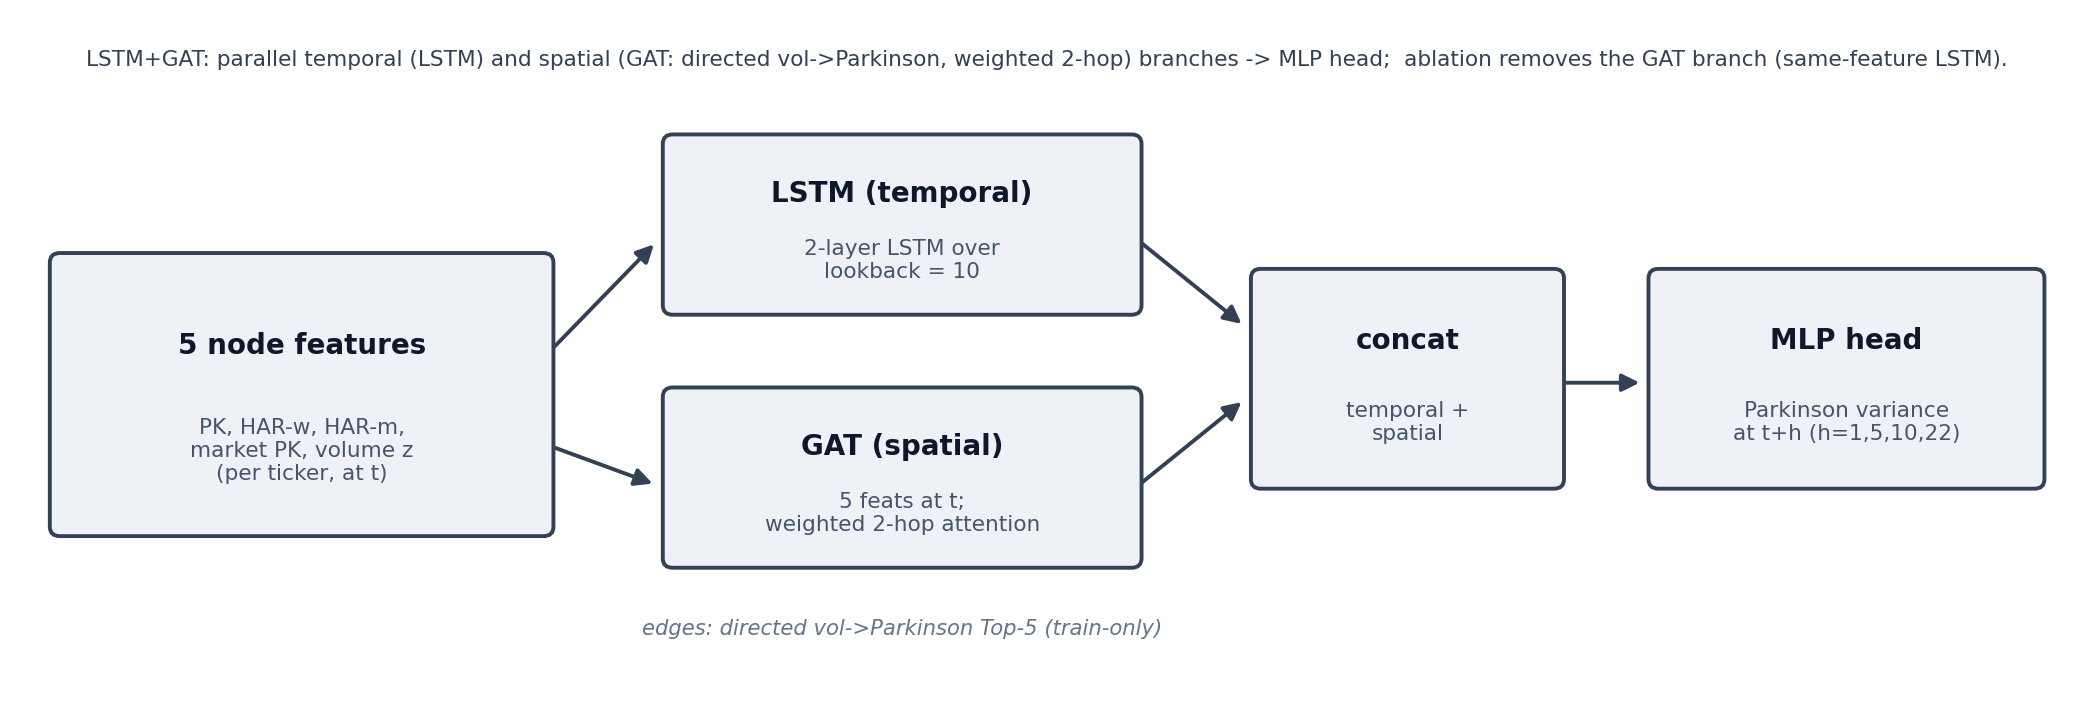
\includegraphics[width=\textwidth]{diagrams/soict_harlstmgat.png}
\caption{VolGA: a per-node LSTM temporal branch and a GAT spatial branch (directed volume$\to$Parkinson
Top-5 weighted two-hop attention) are concatenated into an MLP head; removing the GAT branch gives the
same-feature no-graph LSTM.}
\label{fig:arch}
\end{figure}

\section{Data}
The primary test markets are the \textbf{VN30} (31 screened tickers) and \textbf{VN100} (102 screened
tickers) index panels of the Vietnamese market. Both use the masked panel of Sec.~3 with the five
features, per-ticker standardization fit on training rows only, and the walk-forward protocol above.
The main target is the Parkinson variance; the windowed Yang--Zhang and Rogers--Satchell estimators
appear in an ablation. The VN30 test sample is 10{,}881 masked observations over 351 out-of-sample
dates at $h1$; the VN100 test sample is 46{,}308 masked observations over 454 out-of-sample dates at
$h1$.

\section{Experiments}
The main comparison is HAR, HAR-X, a no-graph LSTM and the proposed model VolGA (directed
volume$\to$Parkinson weighted two-hop) on the VN30 and VN100 panels at horizons $\{1,5,10,22\}$,
reporting MSE, RMSE, MAE and QLIKE and the date-clustered Diebold--Mariano test. The ablations remove
the graph branch (the same-feature no-graph LSTM) and examine widening the deep model's training
universe (Sec.~\ref{sec:pool}); the alternative-estimator and additional-market studies
(Sec.~\ref{sec:est}) are reported as far as the current runs allow.

\section{Results: VN30 and VN100}\label{sec:results}
Tables~\ref{tab:vn30}--\ref{tab:vn100} report all four metrics on the two panels. Lower is better on
MSE, RMSE, MAE and QLIKE; higher is better on $R^2$. The best model per metric column is in bold; for
the learned models the QLIKE is reported as the seed mean $\pm$ the per-seed standard deviation.

\begin{table}[t]
\centering
\caption{VN30 panel (31 nodes; 10{,}881 masked obs over 351 test dates at $h1$; 22 walk-forward folds,
5 seeds; learned models: seed mean, QLIKE $\pm$~per-seed std). Lower is better except $R^2$.
MSE $\times10^{-7}$, RMSE/MAE $\times10^{-4}$.}
\label{tab:vn30}
\footnotesize
\setlength{\tabcolsep}{5pt}
\begin{tabular}{llccccc}
\toprule
$h$ & Model & MSE & RMSE & MAE & QLIKE & $R^2$ \\
\midrule
1 & HAR   & 1.947 & 4.413 & 2.431 & \textbf{0.4952} & 0.2271 \\
1 & HAR-X & 1.938 & 4.402 & 2.402 & 0.4967 & 0.2310 \\
1 & LSTM  & 1.905 & 4.365 & 2.378 & 0.5219\,$\pm$.016 & 0.2439 \\
1 & VolGA & \textbf{1.890} & \textbf{4.348} & \textbf{2.362} & 0.5146\,$\pm$.006 & \textbf{0.2497} \\
\midrule
5 & HAR   & 2.171 & 4.659 & 2.637 & 0.5944 & 0.1453 \\
5 & HAR-X & 2.156 & 4.644 & 2.614 & \textbf{0.5937} & 0.1511 \\
5 & LSTM  & \textbf{2.130} & \textbf{4.616} & \textbf{2.564} & 0.6327\,$\pm$.022 & \textbf{0.1613} \\
5 & VolGA & 2.135 & 4.621 & 2.573 & 0.6150\,$\pm$.023 & 0.1595 \\
\midrule
10 & HAR   & 2.367 & 4.865 & 2.784 & 0.6412 & 0.1066 \\
10 & HAR-X & 2.363 & 4.861 & 2.771 & 0.6394 & 0.1083 \\
10 & LSTM  & \textbf{2.351} & \textbf{4.849} & 2.778 & \textbf{0.6336}\,$\pm$.004 & \textbf{0.1125} \\
10 & VolGA & 2.358 & 4.856 & \textbf{2.758} & 0.6485\,$\pm$.098 & 0.1101 \\
\midrule
22 & HAR   & 2.756 & 5.250 & 3.017 & 0.7012 & 0.0682 \\
22 & HAR-X & \textbf{2.751} & \textbf{5.245} & 3.015 & \textbf{0.6987} & \textbf{0.0699} \\
22 & LSTM  & 2.823 & 5.313 & \textbf{3.010} & 0.7056\,$\pm$.005 & 0.0456 \\
22 & VolGA & 2.829 & 5.319 & 3.011 & 0.7053\,$\pm$.004 & 0.0434 \\
\bottomrule
\end{tabular}
\end{table}

\begin{table}[t]
\centering
\caption{VN100 panel (102 nodes; 46{,}308 masked obs over 454 test dates at $h1$; 22 walk-forward
folds, 5 seeds; learned models: seed mean, QLIKE $\pm$~per-seed std). Same scaling as
Table~\ref{tab:vn30}.}
\label{tab:vn100}
\footnotesize
\setlength{\tabcolsep}{5pt}
\begin{tabular}{llccccc}
\toprule
$h$ & Model & MSE & RMSE & MAE & QLIKE & $R^2$ \\
\midrule
1 & HAR   & 2.369 & 4.867 & 2.906 & 0.4983 & 0.2229 \\
1 & HAR-X & 2.363 & 4.861 & 2.850 & 0.5004 & 0.2248 \\
1 & LSTM  & 2.355 & 4.853 & 2.821 & 0.5025\,$\pm$.020 & 0.2275 \\
1 & VolGA & \textbf{2.348} & \textbf{4.846} & \textbf{2.816} & \textbf{0.4916}\,$\pm$.004 & \textbf{0.2297} \\
\midrule
5 & HAR   & 2.625 & 5.123 & 3.151 & 0.5671 & 0.1403 \\
5 & HAR-X & \textbf{2.602} & \textbf{5.101} & 3.113 & \textbf{0.5610} & \textbf{0.1477} \\
5 & LSTM  & 2.621 & 5.119 & 3.068 & 0.5763\,$\pm$.015 & 0.1416 \\
5 & VolGA & 2.615 & 5.114 & \textbf{3.067} & 0.5705\,$\pm$.013 & 0.1436 \\
\midrule
10 & HAR   & 2.752 & 5.246 & 3.269 & 0.6005 & 0.0986 \\
10 & HAR-X & \textbf{2.748} & \textbf{5.242} & 3.247 & \textbf{0.6001} & \textbf{0.1001} \\
10 & LSTM  & 2.767 & 5.261 & \textbf{3.185} & 0.6096\,$\pm$.028 & 0.0936 \\
10 & VolGA & 2.774 & 5.267 & 3.192 & 0.6149\,$\pm$.033 & 0.0916 \\
\midrule
22 & HAR   & 2.885 & 5.371 & 3.425 & 0.6392 & 0.0565 \\
22 & HAR-X & \textbf{2.883} & \textbf{5.370} & 3.428 & \textbf{0.6388} & \textbf{0.0570} \\
22 & LSTM  & 2.921 & 5.404 & 3.370 & 0.6479\,$\pm$.007 & 0.0448 \\
22 & VolGA & 2.913 & 5.397 & \textbf{3.352} & 0.6434\,$\pm$.003 & 0.0473 \\
\bottomrule
\end{tabular}
\end{table}

On both panels the linear HAR-X keeps the best point QLIKE at most horizons (VN30 at $h5$ and $h22$
and closely at $h10$; VN100 at $h5$, $h10$ and $h22$), consistent with its standing as a hard-to-beat
benchmark. VolGA has the lowest point QLIKE only on VN100 at $h1$. The date-clustered contrasts of
VolGA against HAR-X (Table~\ref{tab:dm}) confirm that no learned model has a significantly lower QLIKE
than HAR-X at any horizon on either panel; where the deep models measurably differ from HAR-X is the
absolute error, where VolGA is significantly lower at the short horizons.

\begin{table}[t]
\centering
\caption{Date-clustered DM contrasts of VolGA vs HAR-X on the two panels, on QLIKE and MAE ($p$-value;
the favoured model in parentheses; bold when $p<0.05$; unadjusted). No QLIKE cell reaches
significance; the significant cells are all MAE reductions by VolGA at the short horizons.}
\label{tab:dm}
\footnotesize
\setlength{\tabcolsep}{5pt}
\begin{tabular}{llcc}
\toprule
Panel & $h$ & QLIKE & MAE \\
\midrule
VN30 & 1 & 0.157 (HAR-X) & \textbf{0.002 (VolGA)} \\
     & 5 & 0.397 (HAR-X) & \textbf{0.009 (VolGA)} \\
     & 10 & 0.717 (HAR-X) & 0.435 (VolGA) \\
     & 22 & 0.788 (HAR-X) & 0.874 (VolGA) \\
\midrule
VN100 & 1 & 0.177 (VolGA) & \textbf{$<$0.001 (VolGA)} \\
      & 5 & 0.585 (HAR-X) & \textbf{0.005 (VolGA)} \\
      & 10 & 0.520 (HAR-X) & \textbf{0.032 (VolGA)} \\
      & 22 & 0.842 (HAR-X) & 0.094 (VolGA) \\
\bottomrule
\end{tabular}
\end{table}

\FloatBarrier
\section{Ablation studies}\label{sec:abl}
\subsection{Graph component}
Removing the GAT branch gives the same-feature no-graph LSTM; the date-clustered DM contrast of VolGA
against it on QLIKE isolates the graph's marginal value (Table~\ref{tab:abl-graph}). The graph adds a
significant QLIKE gain over the no-graph LSTM only on the VN100 panel at the daily horizon
($h1$: $p=0.008$) and the weekly horizon ($h5$: $p=0.011$); on VN30 the graph-vs-LSTM QLIKE contrast
is not significant at any horizon, even though VN30 has the higher mean pairwise correlation. The
reading is that the graph's marginal value tracks node breadth and liquidity rather than
correlation magnitude. The effect is also loss-dependent: on VN30 the graph reaches significance on
absolute error at the daily and ten-day horizons ($p=0.005$ and $p=0.010$) where the QLIKE contrast
does not, so the marginal-value verdict is reported on QLIKE, squared error and absolute error rather
than QLIKE alone. Because the per-seed QLIKE standard deviation of the learned models is in several
cells of the same order as the graph-vs-LSTM difference, the significant graph effect on VN100 is
best read as an ensemble-level regularity at the short horizons rather than a uniform gain.

\begin{table}[t]
\centering
\caption{Graph ablation: date-clustered DM QLIKE contrast of VolGA vs the same-feature no-graph LSTM
($p$-value; the favoured model in parentheses; bold when $p<0.05$; unadjusted).}
\label{tab:abl-graph}
\footnotesize
\setlength{\tabcolsep}{5pt}
\begin{tabular}{lcc}
\toprule
$h$ & VN30 & VN100 \\
\midrule
1  & 0.179 (VolGA) & \textbf{0.008 (VolGA)} \\
5  & 0.112 (VolGA) & \textbf{0.011 (VolGA)} \\
10 & 0.265 (LSTM)  & 0.229 (LSTM) \\
22 & 0.928 (VolGA) & 0.107 (VolGA) \\
\bottomrule
\end{tabular}
\end{table}

\subsection{Widening the training universe (VN30 $\to$ VN100)}\label{sec:pool}
To ask whether the VN30 QLIKE ceiling reflects a shortage of training stocks, we train the deep
models on a single VN100 panel under two arms --- one restricted to the 31 VN30 tickers (Arm~0),
one using all 102 VN100 tickers (Arm~1) --- and score both on the identical 31 VN30 out-of-sample
points, with the paired date-clustered DM comparing Arm~1 against Arm~0 (Table~\ref{tab:pool}).
Across horizons the widened universe does not significantly lower QLIKE on VN30 (VolGA: not
significant at any horizon; LSTM: significant only at $h{=}10$), but it significantly reduces the
absolute error at $h{=}1$ through $h{=}10$ for both deep models, an effect that fades by $h{=}22$.
The benefit of pooling is thus loss- and horizon-dependent: it lowers the average point error at
short-to-medium horizons without translating into a QLIKE gain, consistent with the QLIKE null on
the standalone panels. Only Arm~0 vs Arm~1 is a valid comparison here; Arm~0 is fit on the VN100
grid (with the VN100 market factor) and is not the standalone-VN30 setup of Table~\ref{tab:vn30},
so its numbers are not cross-comparable to that table.

\begin{table}[h]\centering
\caption{Widening the training universe: paired date-clustered DM $p$-values, Arm~1 (VN100-trained)
vs Arm~0 (VN30-trained), both scored on the 31 VN30 stocks over the identical out-of-sample points.
A star marks $p<0.05$ in favour of the wider universe (Arm~1).}\label{tab:pool}
\begin{tabular}{llcccc}
\toprule
Loss & Model & $h{=}1$ & $h{=}5$ & $h{=}10$ & $h{=}22$ \\
\midrule
QLIKE & LSTM & 0.136 & 0.081 & 0.033* & 0.252 \\
QLIKE & VolGA & 0.147 & 0.666 & 0.405 & 0.263 \\
Abs. error & LSTM & $<$0.001* & 0.006* & 0.008* & 0.558 \\
Abs. error & VolGA & $<$0.001* & $<$0.001* & 0.001* & 0.117 \\
\bottomrule
\end{tabular}
\end{table}

\subsection{Alternative volatility estimators}\label{sec:est}
\textbf{[provisional --- full estimator tables pending.]} The Parkinson variance is the chosen
range-based target for this market: prior investigation of the Rogers--Satchell, windowed
Yang--Zhang and close-to-close targets found worse forecast QLIKE, with the loss coming from
non-persistent overnight components that on the unadjusted Vietnamese prices carry corporate-action
jumps; the intraday high--low Parkinson estimator is invariant to price splits and is therefore
preferred. The multi-market, multi-estimator walk-forward tables (Rogers--Satchell and windowed
Yang--Zhang targets across markets) are not yet regenerated on the clean data and are omitted rather
than carried over from earlier runs.
% TODO(coordinator): regenerate estimator tables on clean-data walk-forward before submission.

\subsection{Additional markets}
\textbf{[provisional --- pending clean-data walk-forward.]} Extending the same protocol to the HNX and
HOSE exchanges and the U.S. S\&P 500 as a cross-market comparison is planned; those walk-forward runs
are not yet complete on the current clean data and are intentionally not reported here to avoid
presenting stale numbers as final.
% TODO(coordinator): add HNX / HOSE / S&P 500 clean-data walk-forward when available.

\FloatBarrier
\section{Discussion}\label{sec:disc}
On both Vietnamese panels the picture is a parsimony result. The linear HAR-X retains the best point
QLIKE at most horizons and no learned model is significantly lower on that loss at any horizon
(Table~\ref{tab:dm}); where the deep models measurably differ from HAR-X is the absolute error, on
which VolGA is significantly lower at the short horizons ($h1$ on both panels; also $h5$ on both and
$h10$ on VN100). This is consistent with the difficulty of improving on HAR for actively traded
large-cap panels, where a smooth weighted average of recent volatility is already close to optimal.

\textbf{Graph contribution.} The directed volume$\to$Parkinson graph adds a significant QLIKE gain
over the same-feature no-graph LSTM only on the larger, more liquid VN100 panel at the daily and
weekly horizons (Table~\ref{tab:abl-graph}); on VN30 it is not distinguishable from the no-graph LSTM
on QLIKE at any horizon. Since VN30 carries the higher mean pairwise correlation yet shows the null
graph effect, the graph's marginal value appears to scale with the number of nodes and their
liquidity --- how many stable, informative edges the attention can draw on --- rather than with
correlation magnitude. Because the per-seed QLIKE dispersion of the learned models is in several
cells of the same order as the graph-vs-LSTM difference, and the DM test is computed on the five-seed
ensemble forecast, the significant VN100 graph effect is best read as an ensemble-level regularity at
the short horizons.

\textbf{Loss dependence and multiplicity.} The ranking is metric- and horizon-dependent, which is why
all four metrics are reported with equal weight: the QLIKE comparison is a null result for the deep
models on both panels, while the absolute-error comparison favours VolGA at the short horizons. We
report per-metric DM contrasts without a multiple-comparison correction; the QLIKE null would only be
reinforced by a correction, and the significant absolute-error and VN100 graph results are reported
with their exact $p$-values. \textbf{Inference design.} The date-clustered DM test matters for these
conclusions: a naive per-observation test on this cross-sectionally dependent panel inflates the
statistic by roughly the square root of the number of stocks, so a difference that is not significant
per date can appear significant per observation. \textbf{Capacity.} VolGA adds a graph branch and its
parameters to the no-graph LSTM, so this contrast measures the effect of adding the implemented graph
branch, not of graph structure at matched capacity.

\section{Limitations}
\emph{Split adjustment.} The raw Vietnamese prices are not split- or dividend-adjusted, so
overnight-based estimators inherit corporate-action jumps; we mitigate this by targeting the intraday
high--low Parkinson estimator, which is split-invariant, but the root fix would be adjusted prices.
\emph{Variance target.} The forecasting target is a variance ($\sigma^2$), not a standard deviation
($\sigma$); QLIKE is applied to the variance with a positivity floor taken from the canonical
configuration, and forecast-error magnitudes are on the variance scale. \emph{Floor sensitivity.} The
QLIKE positivity floor interacts with high-zero-range days; floor sensitivity is more pronounced on
illiquid markets and is a documented caveat for any extension to such panels. \emph{Small $N$.} VN30
has only 31 nodes, so deep and graph methods are data-limited there, which is one reason the graph
effect is weaker on VN30 than on the 102-node VN100. \emph{Scope.} The evidence is a
Vietnamese-market case study on two index panels; the additional-market and alternative-estimator
studies are provisional pending completion, and we do not generalise beyond the panels reported.

\section{Conclusion}
On the VN30 and VN100 panels of the Vietnamese market we benchmarked a linear HAR and HAR-X against a
no-graph LSTM and the temporal--graph VolGA model under one leakage-free walk-forward protocol with
the same features and a date-clustered Diebold--Mariano test. Across both panels and all four
horizons no deep model attains a significantly lower QLIKE than the HAR-X benchmark, which keeps the
best point QLIKE at most horizons; the deep models' measurable advantage is a significant reduction in
absolute error at the short horizons. The directed volume$\to$Parkinson graph adds a significant QLIKE
gain over the same-feature no-graph LSTM only on the larger, more liquid VN100 panel at the daily and
weekly horizons and is indistinguishable from the no-graph LSTM on VN30, indicating that the graph's
marginal value tracks node breadth and liquidity rather than correlation magnitude, and that the
verdict is loss-function dependent. The practical takeaway is that, on these Vietnamese index panels,
the added complexity of the deep and graph models does not improve on the linear HAR-X benchmark on
the primary QLIKE loss, and the graph branch earns its keep only on the broader, more liquid panel at
the short horizons.

\begin{thebibliography}{99}
\bibitem{corsi2009} Corsi, F.: A simple approximate long-memory model of realized volatility. J. Financial Econometrics \textbf{7}(2), 174--196 (2009)
\bibitem{parkinson1980} Parkinson, M.: The extreme value method for estimating the variance of the rate of return. J. Business \textbf{53}(1), 61--65 (1980)
\bibitem{yangzhang2000} Yang, D., Zhang, Q.: Drift-independent volatility estimation based on high, low, open, and close prices. J. Business \textbf{73}(3), 477--491 (2000)
\bibitem{rogers1991} Rogers, L.C.G., Satchell, S.E.: Estimating variance from high, low and closing prices. Ann. Appl. Probab. \textbf{1}(4), 504--512 (1991)
\bibitem{lstm1997} Hochreiter, S., Schmidhuber, J.: Long short-term memory. Neural Computation \textbf{9}(8), 1735--1780 (1997)
\bibitem{gat2018} Veli\v{c}kovi\'c, P., et al.: Graph attention networks. In: ICLR (2018)
\bibitem{dm1995} Diebold, F.X., Mariano, R.S.: Comparing predictive accuracy. J. Business \& Economic Statistics \textbf{13}(3), 253--263 (1995)
\bibitem{hln1997} Harvey, D., Leybourne, S., Newbold, P.: Testing the equality of prediction mean squared errors. Int. J. Forecasting \textbf{13}(2), 281--291 (1997)
\bibitem{patton2011} Patton, A.J.: Volatility forecast comparison using imperfect volatility proxies. J. Econometrics \textbf{160}(1), 246--256 (2011)
\bibitem{harq2016} Bollerslev, T., Patton, A.J., Quaedvlieg, R.: Exploiting the errors: a simple approach for improved volatility forecasting. J. Econometrics \textbf{192}(1), 1--18 (2016)
\bibitem{chen2022} Chen, Q., Robert, C.-Y.: Multivariate realized volatility forecasting with graph neural network. In: ACM ICAIF (2022). arXiv:2112.09015
\bibitem{gnnhar2025} Zhang, C., Pu, X., Cucuringu, M., Dong, X.: Forecasting realized volatility with spillover effects: perspectives from graph neural networks (2025). arXiv:2308.01419
\bibitem{dy2012} Diebold, F.X., Yilmaz, K.: Better to give than to receive: predictive directional measurement of volatility spillovers. Int. J. Forecasting \textbf{28}(1), 57--66 (2012)
\bibitem{audrino2025} Audrino, F., Chassot, J.: HARd to beat: the overlooked impact of rolling windows in the era of machine learning. Int. J. Forecasting (2025). arXiv:2406.08041
\bibitem{clements2024} Clements, A., Preve, D., Tee, C.-Z.: Harvesting the HAR-X: forecasting volatility with low-frequency OHLC data (2024)
\bibitem{gnarharx2025} GNAR-HARX: a network-augmented HAR-X model for realized volatility (2025). arXiv:2510.24443
\end{thebibliography}

\end{document}
